\documentclass[11pt,a4paper]{article}

% ============================================================================
%  How Predictable Are Rare Precipitation Extremes?
%  A Calibration-Aware Assessment for London and Paris
%
%  Predictability assessment + evaluation methodology. Results in
%  ../04_prototype_results.md; figures built by figures/make_figs.py and
%  figures/make_horizon_fig.py.
%  Compile:  pdflatex main ; bibtex main ; pdflatex main ; pdflatex main
% ============================================================================

\usepackage[T1]{fontenc}
\usepackage[utf8]{inputenc}
\usepackage{lmodern}
\usepackage{microtype}
\usepackage[a4paper,margin=2.5cm]{geometry}
\usepackage{amsmath,amssymb,amsthm,bm}
\usepackage{mathtools}
\usepackage{graphicx}
\usepackage{booktabs}
\usepackage{xcolor}
\usepackage{caption}
\usepackage[round,authoryear]{natbib}
\usepackage[hidelinks]{hyperref}
\usepackage{enumitem}

% ---- theorem environments ----
\newtheorem{theorem}{Theorem}
\newtheorem{proposition}{Proposition}
\newtheorem{assumption}{Assumption}
\newtheorem{definition}{Definition}
\newtheorem{remark}{Remark}

% ---- notation macros ----
\newcommand{\Ind}{\mathcal{I}}                 % precipitation index
\newcommand{\GP}{\mathcal{GP}}
\newcommand{\Real}{\mathbb{R}}
\newcommand{\E}{\mathbb{E}}
\newcommand{\Prob}{\mathbb{P}}
\newcommand{\Normal}{\mathcal{N}}
\newcommand{\GPD}{\mathrm{GPD}}
\newcommand{\sigmoid}{\operatorname{sigmoid}}
\newcommand{\softplus}{\operatorname{softplus}}
\newcommand{\KL}{\mathrm{KL}}
\newcommand{\bx}{\bm{x}}
\newcommand{\bg}{\bm{g}}
\newcommand{\bff}{\bm{f}}
\newcommand{\bB}{\bm{B}}
\newcommand{\bK}{\bm{K}}
\newcommand{\bu}{\bm{u}}
\newcommand{\bZ}{\bm{Z}}
\newcommand{\Filt}{\mathcal{F}}
\DeclareMathOperator*{\argmax}{arg\,max}
\DeclareMathOperator*{\argmin}{arg\,min}

\title{\bfseries How Predictable Are Rare Precipitation Extremes?\\
A Calibration-Aware Assessment for London and Paris}
\author{Olatunji Johnson\\[0.3em]
\small Department of Mathematics, University of Manchester\\[0.2em]
\small Corresponding author: Olatunji Johnson
(\href{mailto:olatunji.johnson@manchester.ac.uk}{\texttt{olatunji.johnson@manchester.ac.uk}})}
\date{\today}

\begin{document}
\maketitle

\begin{abstract}
\noindent
How predictable are rare precipitation extremes, and how should that
predictability be measured? We address both questions using thirty years
(1989--2018) of a standardised precipitation-extreme index for London
(maritime) and Paris (more continental), with strictly antecedent ERA5
drivers. We argue rare-event forecasts must be judged by
\emph{calibration-aware proper scores} against climatology, and assemble a
protocol (Brier decomposition, threshold-weighted CRPS skill,
bootstrap intervals, multi-split checks) guarding against the single-seed and
quantile-selection pitfalls that inflate apparent skill. Across a bake-off from
logistic regression to a Gaussian-process extreme-value hurdle, we find, consistently in both cities, that (i) the Gaussian-process
hurdle is the most skilful full-distribution forecaster on the
tail, while simple calibrated models (logistic regression,
gradient-boosted trees) match it on occurrence, and the choice of response
distribution matters as much as model class --- a zero-inflated log-normal is
catastrophically miscalibrated where a threshold-free extended generalised Pareto
distribution is not; (ii) occurrence is weakly but genuinely predictable from
antecedent convective instability and circulation; and (iii) the
magnitude of the largest events is weakly but robustly predictable from
convective instability (CAPE/CIN), with a CRPS skill over climatology excluding
zero across four independent splits per city. The effects are small,
statistically robust, and physically plausible; replication across two cities
that share the same reanalysis source offers modest, not decisive, evidence
against a location-specific artefact.
\end{abstract}

\noindent\textbf{Keywords:} extreme-value theory; proper scoring rules; forecast
verification; conformal prediction; Gaussian processes; convective instability.

% ===========================================================================
\section{Introduction}\label{sec:intro}
% ===========================================================================

Extreme precipitation is among the most damaging natural hazards facing
temperate cities. Short, intense rainfall episodes trigger surface-water and
river flooding, disrupt transport, overwhelm drainage, and impose large and
unevenly distributed economic and social costs. In cities such as London and
Paris such events occur on only a small fraction of days, yet a single episode can
cause disproportionate
harm, and both observational records and climate projections indicate that the
frequency and intensity of heavy rainfall are increasing \citep{ipcc2021}.
Skilful and, above
all, \emph{trustworthy} early warning of these events would let emergency
managers, infrastructure operators, and insurers act pre-emptively. This
motivates probabilistic forecasts of extreme precipitation at horizons of days
to weeks ahead.

The statistical obstacles are severe. Extreme days are rare, typically
a few percent of the record, so a model that simply predicts ``no extreme'' is
accurate yet useless, and conventional accuracy is the wrong yardstick. The
daily precipitation index is zero-inflated, strongly right-skewed, and
heavy-tailed, violating the Gaussian assumptions underlying standard regression.
The observational record is short relative to the rarity of the events, leaving
few positive examples from which to learn, and the day-to-day persistence of
extremes is limited, so intrinsic predictability is modest. Together these
features cap raw forecast \emph{skill}, a ceiling any honest treatment must
confront rather than obscure.

We argue that, precisely because raw predictability is limited, the decisive
quality of a forecast in this setting is not discrimination but
\emph{calibration}: whether the issued probabilities can be trusted. A forecast
that assigns a $5\%$ probability to an extreme is useful for decision-making
only if extremes do occur on about $5\%$ of such days; an overconfident forecast
that systematically overstates rare-event probabilities causes false alarms and
wasted resources, while an underconfident one breeds complacency. The
appropriate goal is therefore to \emph{maximise sharpness subject to
calibration} \citep{gneiting2007sharpness}: to be as informative as the data
allow while remaining honest. Calibration matters most exactly where it is
hardest to achieve --- in the tail --- and evaluating it there is itself subtle,
as the \emph{forecaster's dilemma} makes clear \citep{lerch2017dilemma}.

No existing methodology delivers calibrated, guaranteed tail probabilities for
rare-event forecasting, because the three relevant tools each supply only part
of the answer. \emph{Extreme-value theory} (EVT) furnishes asymptotically
justified tail models, but is most often used descriptively, for return
levels or non-stationary tail regression, rather than for flexible,
covariate-driven probabilistic forecasting, and it offers no finite-sample
coverage guarantee \citep{coles2001evt,davison1990}. \emph{Flexible machine
learning}, including deep models and Gaussian processes, captures non-linear
dependence on atmospheric predictors and yields predictive distributions, but
those distributions are typically miscalibrated in the tail and come with no
guarantee \citep{galib2022deepextrema,lakshminarayanan2017}. Conformal prediction provides distribution-free, finite-sample coverage, but its standard form does not guarantee conditional or tail-specific coverage --- the effective resolution of very high quantiles is limited by the size of the calibration set --- and assumes exchangeability, which is generally violated in daily time series due to temporal dependence and non-stationarity \citep{gibbs2021adaptive,pasche2025extreme}. Moreover, many two-part (hurdle) forecasting approaches estimate occurrence and intensity in separate stages, so that inference about extremes relies primarily on the relatively small number of exceedances. This separation can limit the extent to which information contained in the abundant non-extreme data informs tail inference, particularly when common latent processes govern both occurrence and intensity.

Rather than advocate a single model, we therefore ask a more basic pair of
questions --- \emph{how predictable are these extremes, and how should that
predictability be measured?} --- and answer them with a careful evaluation
protocol and a bake-off of models spanning logistic regression, zero-inflated
distributional regressions (log-normal, gamma, and the threshold-free extended
generalised Pareto distribution), and a Gaussian-process extreme-value
hurdle with conformal calibration.

\paragraph{Contributions.}
\begin{enumerate}[leftmargin=1.6em,itemsep=1pt]
  \item A \textbf{calibration-aware evaluation protocol} for rare-event
  precipitation forecasting: Brier reliability/resolution decomposition,
  threshold- and quantile-weighted CRPS, skill scores against climatology,
  bootstrap confidence intervals, and multi-split robustness --- designed to
  resist the single-seed and quantile-selection artefacts that inflate apparent
  skill, and to demonstrate that conformal coverage is insufficient as a
  stand-alone measure of forecast quality.
  \item A \textbf{rigorous predictability assessment, replicated in two
  contrasting cities}: occurrence of an extreme is weakly but genuinely
  predictable from antecedent state; and the \emph{magnitude} of the largest
  events carries weak but robust predictability tied to antecedent convective
  instability (CAPE/CIN), with a CRPS skill over climatology whose moving-block
  bootstrap interval excludes zero across four independent train/test splits in
  each city --- and is stronger in the more convective Paris, consistent with a
  meteorological rather than a purely local origin (though two cities in one
  climate zone offer only modest evidence on geographic generality).
  \item A \textbf{methodological finding on what matters}: across the bake-off, a
  Gaussian-process extreme-value hurdle is the most skilful full-distribution
  forecaster on the tail in both cities --- and, on occurrence, is matched by an
  inexpensive calibrated logistic regression and gradient-boosted trees --- while
  the choice of response distribution matters as much as model class (a
  zero-inflated log-normal is catastrophically miscalibrated where a threshold-free
  extended GPD is well behaved), and conformal coverage, though attained by
  construction, is insufficient on its own as a measure of forecast quality.
\end{enumerate}

Empirically, we study the daily standardised precipitation index over 1989--2018
for two cities of contrasting climate: London (maritime, $417$ extreme days at the
$95$th percentile) and Paris (more continental and convective, $607$ extreme
days). The $95$th-percentile index is the primary target; the rarer
$99$th-percentile index ($137$ events for London) is too data-scarce for the
held-out intensity analysis (its occurrence-only results are in the Supplementary
Material). Predictors are strictly antecedent ERA5 atmospheric drivers (circulation,
moisture, and convective-instability fields) and large-scale teleconnection
indices. Because the index is itself an ERA5-derived precipitation product, we
exclude all precipitation fields from the predictors and lag every driver, so the
assessment is of genuine antecedent predictability rather than diagnosis.

The remainder of the paper is organised as follows.
Section~\ref{sec:related} positions our work within the literatures on
extreme-value modelling, Gaussian processes, conformal prediction, and forecast
evaluation. Section~\ref{sec:data} describes the data and predictors.
Section~\ref{sec:method} sets out the models we compare, the conformal
calibration, and the evaluation protocol. Section~\ref{sec:results} presents the
results, and Sections~\ref{sec:discussion}--\ref{sec:conclusion} discuss
implications and conclude.

% ===========================================================================
\section{Related work}\label{sec:related}
% ===========================================================================

Our work sits at the intersection of four literatures; we review each in turn and
then state precisely how this study differs.

\paragraph{Statistical modelling of precipitation extremes.}
Extreme-value theory provides the asymptotic foundation for tail modelling. The
peaks-over-threshold approach models exceedances above a high threshold by the
Generalised Pareto distribution \citep{pickands1975,davison1990}, the framework
we adopt for the intensity component; the block-maxima approach uses the
Generalised Extreme Value distribution \citep{coles2001evt}. EVT is widely
applied in hydrology and climatology \citep{katz2002}, including non-stationary
and spatial Bayesian formulations of precipitation extremes
\citep{cooley2007}. This body of work is, however, predominantly
\emph{descriptive} --- estimating return levels or letting tail parameters vary
smoothly with a few covariates --- rather than producing flexible,
covariate-rich \emph{forecasts} at a fixed lead time, and it offers no
finite-sample coverage guarantee. We retain the GPD tail but embed it in a
flexible predictive model and calibrate it conformally.

\paragraph{Machine learning and deep learning for extremes.}
Data-driven methods increasingly target extremes: \citet{galib2022deepextrema}
forecast block maxima with a deep network constrained by GEV theory, and neural
networks have been used to estimate extreme-value parameters. More broadly,
predictive uncertainty in deep models is quantified with deep ensembles
\citep{lakshminarayanan2017} and Monte-Carlo dropout \citep{gal2016}. These
methods capture non-linear dependence on predictors and return uncertainty
estimates, but they are typically miscalibrated in the tail and lack
distribution-free guarantees --- the gap our conformal layer closes.

\paragraph{Gaussian processes: scalability and multiple outputs.}
Gaussian processes offer principled non-parametric regression with built-in
uncertainty \citep{rasmussen2006gpml}, made scalable through sparse variational
inference with inducing points \citep{titsias2009,hensman2013,salimbeni2017doubly}.
Expressiveness can be increased by composing layers in deep Gaussian processes
\citep{damianou2013deep} or by learning the kernel through a neural feature
map in deep kernel learning \citep{wilson2016deepkernel}, though --- as we find
below --- such added depth is not warranted on our low-signal, single-site
problem. Correlated outputs are
modelled by multi-output GPs and coregionalisation
\citep{bonilla2008multitask,alvarez2012kernels}. A GP with a Gaussian likelihood
cannot represent heavy-tailed, skewed, zero-inflated responses; we therefore
pair the GP prior with an EVT likelihood and use coregionalisation not to share
information across tasks but to couple the two halves of a hurdle model.

\paragraph{Two-part, hurdle, and selection models.}
Semicontinuous and zero-inflated outcomes are commonly modelled by two-part
(hurdle) decompositions separating occurrence from intensity. Allowing the two
parts to be \emph{dependent} has a long history: correlated random-effects
formulations \citep{olsen2001twopart}, copula couplings, and the sample-selection
models of econometrics \citep{heckman1979selection}, which explicitly address the
correlation between a selection (occurrence) equation and an outcome (intensity)
equation. To our knowledge this dependence has not been exploited within a
GP--EVT \emph{forecasting} model, where --- because intensity is observed
only on the rare extreme days --- borrowing strength from the abundant
occurrence data is a natural idea; we implement and test it, and report (in the
Supplementary Material) that at this data volume the coupling is weakly identified
and empirically inert.

\paragraph{Conformal prediction.}
Conformal prediction yields distribution-free, finite-sample coverage for any
underlying predictor \citep{vovk2005}. Split-conformal methods make this
practical for regression \citep{lei2018}, and conformalised quantile regression
adapts the intervals to heteroscedasticity \citep{romano2019cqr}. Exchangeability
can be relaxed for covariate shift \citep{tibshirani2019} and, crucially for us,
for time series and online distribution shift through adaptive conformal
inference \citep{gibbs2021adaptive,xu2021}. Coverage at very high confidence
levels --- the extreme regime --- is addressed by \citet{pasche2025extreme}, who
combine EVT with conformal prediction to build reliable intervals for
high-impact events. That work, the closest to ours, constructs \emph{regression
intervals} from a black-box extreme-quantile estimator under (weighted)
exchangeability; it uses neither a Gaussian-process nor a generative model, does
not forecast exceedance \emph{probabilities}, and does not model temporal
dependence natively. Here, by contrast, tail-targeted and temporally-adaptive
conformal calibration is applied to a generative model, within a broader
predictability study.

\paragraph{Forecast evaluation of extremes.}
Probabilistic forecasts are assessed with proper scoring rules
\citep{gneiting2007scoring} under the paradigm of maximising sharpness subject to
calibration \citep{gneiting2007sharpness}; the Brier score admits a
reliability--resolution decomposition \citep{murphy1973}. For extremes,
threshold- and quantile-weighted scoring rules focus evaluation on the tail
while remaining proper \citep{gneiting2011threshold}, and naive restriction to
extreme observations can paradoxically reward miscalibrated forecasts --- the
forecaster's dilemma \citep{lerch2017dilemma}. Our evaluation is built on these
principles.

\paragraph{Positioning.}
Much of this literature proposes ever more expressive models for extremes. We
take the complementary stance of \emph{measuring} how much is predictable and
which modelling choices matter, under an evaluation protocol built from proper
scoring rules, skill against climatology, and bootstrap and multi-split
robustness. In doing so we find --- against the prevailing direction --- that
under this dataset and evaluation framework a compact Gaussian-process
extreme-value hurdle is the most skilful full-distribution forecaster on the tail
in both cities, yet simple calibrated models match it on occurrence, so raw model
sophistication buys little here. We also find that conformal coverage,
increasingly reported as a calibration guarantee, is insufficient on its own as a
measure of forecast quality. This emphasis on rigorous
predictability assessment, rather than a new architecture, is the gap we fill.

% ===========================================================================
\section{Data}\label{sec:data}
% ===========================================================================

\subsection{The precipitation-extreme index}\label{sec:data-index}
Our response variable is a standardised daily precipitation-extreme index,
computed for two European cities --- \textbf{London} and \textbf{Paris} ---
derived from the Copernicus Climate Data Store product \emph{Extreme precipitation
risk indicators for Europe and European cities (1950--2019)}. The underlying field
is the ERA5 reanalysis dynamically downscaled to a
$2\,\mathrm{km}\times2\,\mathrm{km}$ grid (ERA5-2km) with urban parameterisation,
which resolves London as $53$ and Paris as $157$ grid cells. For each cell and day
the indicator is the standardised exceedance
\begin{equation}\label{eq:index-def}
\Ind \;=\; \frac{P}{P_q},
\end{equation}
where $P$ is daily precipitation and $P_q$ is the fixed $q$th percentile of wet
days ($P\ge 1\,\mathrm{mm}$) over the 1950--2019 reference period. The index is
dimensionless, and $\Ind>1$ marks an extreme: precipitation exceeding the
historical $q$th-percentile level. To obtain a single city-level series we take the
daily maximum of $\Ind$ over the city's cells, so an extreme day is one on which
\emph{any} part of the city exceeds its threshold. We analyse the thirty-year
record 1989--2018 at the $q=95$ (primary) and $q=99$ thresholds. The two cities
are chosen for their contrasting climates: London's maritime regime versus Paris's
more continental, more convective one --- a deliberate test of whether conclusions
generalise.

\subsection{Exploratory characteristics}\label{sec:data-eda}
The series comprises $10{,}957$ daily observations. Its defining features ---
which directly motivate the modelling choices of Section~\ref{sec:method} ---
are summarised in Table~\ref{tab:data} and Figure~\ref{fig:data}, and are shared
by both cities. First, extremes are \emph{rare}: $3.8\%$ of London days and
$5.5\%$ of Paris days exceed the $95$th-percentile threshold (and only $1.3\%$ at
the $99$th in London). Second, the index is
\emph{zero-inflated and heavy-tailed}: about a quarter of days are exactly zero,
the median is below $0.02$, yet the maximum exceeds $6$ at the $95$th-percentile
standardisation --- a strong right skew incompatible with a Gaussian response.
Third, occurrence is \emph{seasonal}: the monthly extreme rate peaks in summer
(July--August, reaching $6\%$ at the $95$th percentile and $3\%$ at the $99$th)
and is lowest in late winter and early spring, consistent with convective
summer rainfall. Fourth, the extreme indicator exhibits only \emph{limited
temporal autocorrelation}, so the persistence available to an autoregressive
forecaster is modest --- one reason that drivers beyond the index's own history
(Section~\ref{sec:data-predictors}) are essential.

\begin{table}[t]
\centering
\small
\caption{Summary characteristics of the $95$th-percentile precipitation-extreme
index (1989--2018; $N=10{,}957$ days) for the two cities. Extreme days are those
with $\Ind>1$. Paris is more convective: more cells, more extremes, a heavier
tail. (London's $99$th-percentile statistics --- $137$ extreme days --- are used
only in the Supplementary Material.)}
\label{tab:data}
\begin{tabular}{lcc}
\toprule
& \textbf{London} & \textbf{Paris}\\
& {\small(maritime)} & {\small(continental)}\\
\midrule
Grid cells                      & $53$ & $157$\\
Extreme days (total)            & $417$ & $607$\\
Extreme rate (\%)               & $3.81$ & $5.54$\\
\;\;train 1989--2008 ($7{,}305$ d) & $287$ ($3.93\%$) & $396$ ($5.42\%$)\\
\;\;test\phantom{i} 2009--2018 ($3{,}652$ d) & $130$ ($3.56\%$) & $211$ ($5.78\%$)\\
Days equal to zero (\%)         & $25.5$ & $28.7$\\
Median index                    & $0.015$ & $0.012$\\
Maximum index                   & $6.46$ & $8.91$\\
Peak season                     & \multicolumn{2}{c}{July--August}\\
\bottomrule
\end{tabular}
\end{table}
\begin{figure}[t]
\centering
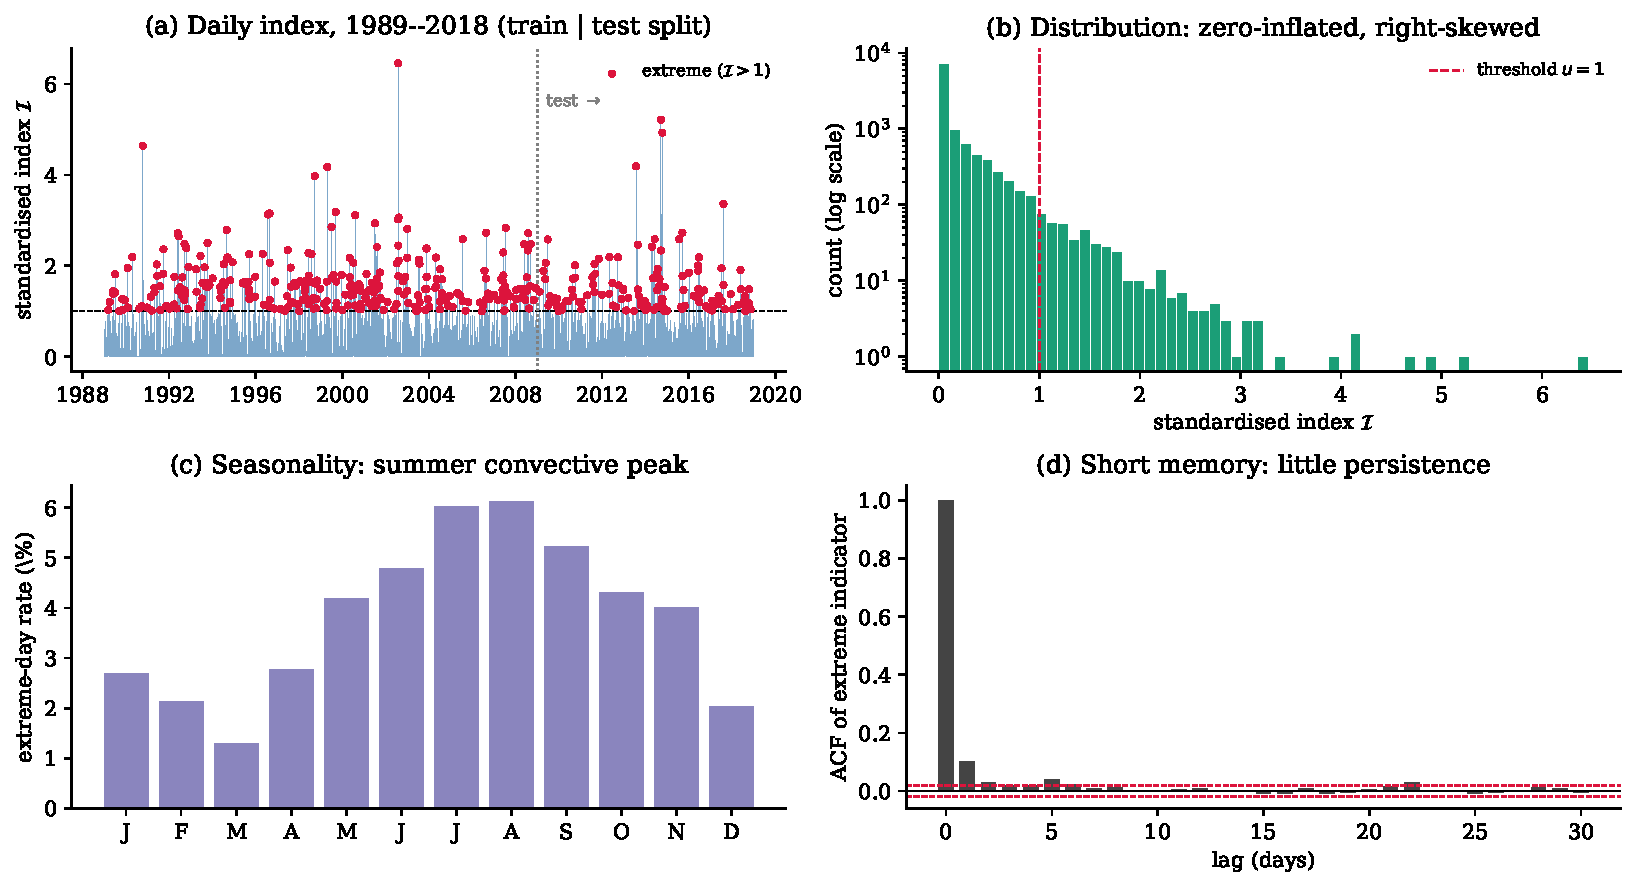
\includegraphics[width=\linewidth]{figures/fig_data}
\caption{The London $95$th-percentile precipitation-extreme index, 1989--2018
(Paris is qualitatively similar; see Supplementary Figure~S1).
\textbf{(a)} Daily series with extreme days ($\Ind>1$) marked and the train/test
split; \textbf{(b)} the distribution is zero-inflated ($\sim$a quarter of days
are exactly zero) and strongly right-skewed (log count); \textbf{(c)} extremes
peak in summer (convective rainfall); \textbf{(d)} the extreme indicator has very
short memory --- the autocorrelation is negligible beyond a day or two (dashed:
$95\%$ band) --- which caps how much an autoregressive forecaster can achieve.}
\label{fig:data}
\end{figure}

\subsection{Antecedent predictors}\label{sec:data-predictors}
All predictors are \emph{strictly antecedent}: for a horizon-$h$ forecast of day
$t+h$ they are functions only of information available up to day $t$. We use
three groups.
\begin{enumerate}[leftmargin=1.6em,itemsep=2pt]
  \item \textbf{Index history.} Lagged values of the index (up to $14$ days),
  rolling means and maxima over $7$/$14$/$30$-day windows, counts of recent
  exceedances, and harmonic encodings of day-of-year and month to capture
  seasonality.
  \item \textbf{ERA5 atmospheric drivers.} Antecedent fields from the ERA5
  reanalysis over a synoptic-scale window around each city: mean sea-level pressure
  and its gradients, geopotential height ($500$/$850\,$hPa), specific and
  total-column water vapour, integrated water-vapour transport, near-surface
  temperature and winds, and convective-instability diagnostics --- convective
  available potential energy (CAPE) and convective inhibition (CIN), the
  K-index, and the Total-Totals index. Fields are aggregated to daily statistics (means, and maxima for the
  convective indices) and reduced to regional summaries.
  \item \textbf{Teleconnection indices.} Lagged North Atlantic Oscillation,
  Arctic Oscillation, and an El Ni\~no--Southern Oscillation index, capturing
  large-scale circulation states relevant at longer horizons.
\end{enumerate}
In total $d=49$ predictors enter the full model: $20$ index-history features
(lags, rolling summaries, and seasonality harmonics), $26$ ERA5 circulation,
moisture, and convective-instability fields, and $3$ teleconnection indices.
In the analysis the drivers are introduced \emph{cumulatively} --- index history;
$+$\,teleconnections; $+$\,ERA5 circulation and moisture; $+$\,convective
instability --- so that each increment isolates a class of predictors. All
features are standardised using training-set statistics only; the complete list
and the retrieval recipe are in Appendix~\ref{app:data}.

\begin{remark}[No leakage; perfect-prognosis framing]
ERA5 is a reanalysis that assimilates observations, so using fields at or after
the target day would be circular. We therefore use only \emph{lagged} drivers,
known strictly before the forecast time. This is the standard
\emph{perfect-prognosis} predictability setting; an operational system would
replace antecedent ERA5 with numerical-weather-prediction \emph{forecast}
fields, which we leave to future work (Section~\ref{sec:conclusion}).
\end{remark}

\subsection{Threshold, training, and testing}\label{sec:data-split}
We take the \textbf{$95$th-percentile index as the primary target}: its $417$
extreme days ($287$ train, $130$ test) admit the full analysis, including the
held-out intensity test, which requires extreme days in both training and test
across several splits. The rarer $99$th-percentile index has only $137$ extreme
days in thirty years ($101$ train, $36$ test) --- too few for the intensity
analysis --- so its occurrence-only results are given in Supplementary
Section~S1 (Table~S1). Unless stated, results are for the $95$th percentile at
horizon $h=1$.

Because the data are a time series, all splits respect chronology. The primary
split trains on 1989--2008 ($7{,}305$ days) and holds out 2009--2018 ($3{,}652$
days); preprocessing statistics and conformal calibration sets are derived from
the training period only. To verify that results are not an artefact of a single
test window, the intensity analysis is additionally repeated over four
forward-only, expanding-window splits (test periods beginning 2003, 2006, 2009,
and 2012), and all stochastic results are averaged over random seeds.

% ===========================================================================
\section{Methodology}\label{sec:method}
% ===========================================================================

Section~\ref{sec:setup} fixes notation and the predictability target.
Section~\ref{sec:models} describes the ladder of models we compare, from
climatology and logistic regression through zero-inflated distributional
regressions to a Gaussian-process extreme-value hurdle.
Section~\ref{sec:conformal} describes the conformal calibration we assess (and
why its coverage guarantee is, on its own, uninformative).
Section~\ref{sec:metrics} sets out the evaluation protocol --- proper scores,
skill against climatology, a hold-out intensity test, and bootstrap and
multi-split robustness --- which is itself a contribution.

% --------------------------------------------------------------------------
\subsection{Problem set-up and notation}\label{sec:setup}
% --------------------------------------------------------------------------
Let $\Ind_t \ge 0$ denote the daily standardised precipitation index on day
$t$, and let $u>0$ be a fixed exceedance threshold (we take $u=1$, the value at
which the index marks an extreme, and report sensitivity to $u$ in
Section~\ref{sec:res-bakeoff}). Because $\Ind=P/P_q$ is itself standardised against the training-period
$q$th percentile (Section~\ref{sec:data-index}), $u$ and $q$ play distinct
roles: $q$ sets which event counts as rare in the first place (e.g.\ the
$99$th-percentile analysis of Section~\ref{sec:data-split}), while $u$ sets
how far above that level counts as extreme --- e.g.\ $u=1.25$ requires
exceeding $125\%$ of the $q$th-percentile level. A day
is
\emph{extreme} when $\Ind_t > u$. Write the occurrence indicator and the excess
as
\begin{equation}
O_t \;=\; \mathbf{1}\{\Ind_t > u\},
\qquad
Y_t \;=\; (\Ind_t - u)\,\big|\,\{\Ind_t > u\},
\end{equation}
so that $O_t\in\{0,1\}$ is observed every day while the excess $Y_t$ is
\emph{defined and observed only on extreme days}. This asymmetry --- many
occurrence observations, few intensity observations --- shapes both the modelling
(Section~\ref{sec:models}) and the separate evaluation of occurrence and
intensity predictability (Section~\ref{sec:metrics}).

Each day carries a vector of covariates $\bx_t\in\Real^d$ that are
\emph{strictly antecedent}: functions of information available up to and
including day $t$ (autoregressive lags and rolling summaries of the index, plus
lagged ERA5 atmospheric drivers and teleconnection indices; see
Section~\ref{sec:data}). Let $\Filt_t$ be the filtration generated by all
information up to day $t$. For a forecast horizon $h\ge 1$ the target is the
\emph{predictive distribution} of $\Ind_{t+h}$ given $\Filt_t$, summarised by
its conditional CDF
\begin{equation}
F_{t+h}(z) \;=\; \Prob\!\left(\Ind_{t+h} \le z \,\middle|\, \Filt_t\right),
\qquad z\ge 0 .
\end{equation}
Two functionals are of primary interest: the \emph{exceedance probability}
$\pi_{t+h}=\Prob(\Ind_{t+h}>u\mid\Filt_t)=1-F_{t+h}(u)$ and the conditional law
of the excess $Y_{t+h}\mid\{\Ind_{t+h}>u\}$.

% --------------------------------------------------------------------------
\subsection{Models compared}\label{sec:models}
% --------------------------------------------------------------------------
We assess a ladder of models of increasing complexity, all sharing the same
strictly antecedent covariates $\bx_t$ and judged by the protocol of
Section~\ref{sec:metrics}. The aim is not to crown one architecture but to learn
\emph{how much} of the index is predictable and \emph{which} modelling choices
matter.
Models fall into two groups: \emph{occurrence-only classifiers} (which estimate only the exceedance probability~$\pi_{t+h}$, and are not scored on the full distribution) and \emph{full-distribution models} (which output the complete CDF $F_{t+h}$ and are additionally evaluated with the tail-CRPS of Section~\ref{sec:metrics}).

\paragraph{Baselines.} \emph{Climatology} issues the empirical distribution of
the training index, the reference against which every skill score is measured; a
\emph{stationary peaks-over-threshold} (POT) model adds a Generalised Pareto tail
fitted to the training excesses but no covariate dependence.

\paragraph{Occurrence: logistic regression and gradient-boosted trees.} For the
exceedance probability $\pi_{t+h}=\Prob(\Ind_{t+h}>u\mid\Filt_t)$ we fit a
regularised logistic regression on $\bx_t$ --- the natural calibrated occurrence
model --- and, as a strong non-linear machine-learning baseline, an
isotonic-calibrated gradient-boosted-tree classifier (XGBoost).

\paragraph{Full-distribution zero-inflated regression.} Rather than hurdle at the
extreme threshold --- which restricts intensity estimation to the few
exceedances --- we model the \emph{entire} distribution of $\Ind$ using all wet
days and derive the exceedance probability and tail from it. With a point mass
$p_0(\bx_t)$ at zero and a positive continuous CDF $F_+$,
\begin{equation}\label{eq:zi}
F_{t+h}(z) = p_0 + (1-p_0)\,F_+\!\big(z;\bm\theta(\bx_t)\big)\ (z>0),
\qquad \pi_{t+h}=(1-p_0)\big(1-F_+(u)\big),
\end{equation}
with $p_0(\bx_t) = \mathrm{sigmoid}(\mathbf{w}_0^\top\bx_t)$ and the distribution parameters $\bm\theta(\bx_t) = \mathrm{link}(\mathbf{W}\bx_t)$ driven by linear predictors in $\bx_t$.
The Generalised Pareto distribution (GPD) is
\begin{equation}\label{eq:gpd}
H(y;\sigma,\xi) = 1-\left(1+\xi y/\sigma\right)_{+}^{-1/\xi}\ (\xi\neq0),\quad
1-e^{-y/\sigma}\ (\xi=0),\quad y\ge0,
\end{equation}
with $(a)_+=\max(a,0)$ and $\xi$ governing tail heaviness. For $F_+$ we compare three choices: (i)~a \emph{log-normal}, (ii)~a \emph{gamma}, and (iii)~the \emph{extended GPD} (eGPD) --- the extreme-value-motivated choice ---
\begin{equation}\label{eq:egpd}
F_+(z) = \big[H(z;\sigma,\xi)\big]^{\kappa},\qquad \kappa>0,
\end{equation}
which is GPD-tailed at high values (inheriting the Pickands--Balkema--de Haan
justification of extreme-value theory; \citealp{coles2001evt}) yet is a single
continuous model over all positive intensities, requiring \emph{no} threshold
selection ($\kappa$ shapes the lower tail).

\paragraph{Hurdle with a GPD tail: a Gaussian-process variant.} The most flexible
contender is a two-part hurdle whose intensity component is a
non-stationary GPD,
\begin{equation}\label{eq:hurdle-cdf}
F_{t+h}(z) = (1-\pi_{t+h}) + \pi_{t+h}\,H(z-u;\sigma_{t+h},\xi),\qquad z>u,
\end{equation}
with $\pi_{t+h}=\sigmoid(g_\pi(\bx_t))$ and
$\sigma_{t+h}=\softplus(g_\sigma(\bx_t))$ driven by latent functions $g_\pi,
g_\sigma$ on which we place Gaussian-process priors --- a single-layer GP with a
standard automatic-relevance-determination squared-exponential kernel acting
directly on the covariates, fitted by sparse variational inference
\citep{salimbeni2017doubly}. We refer to it as the \emph{GP--EVT hurdle}
throughout (Table~\ref{tab:bakeoff}). A Gaussian-likelihood
GP cannot represent the zero-inflation and heavy tail of $\Ind$, which motivates
the EVT likelihood. Full inference details are in Appendix~\ref{app:inference}.

\paragraph{Dependent hurdle: coupling occurrence and intensity.} The classical
hurdle assumes occurrence and intensity are conditionally independent; physically
they should be positively correlated, and coupling them could let the abundant
occurrence data inform the data-starved tail. In
plain terms: rather than fitting the occurrence function $g_\pi$ and the
intensity function $g_\sigma$ independently, we let $g_\sigma$ borrow
statistical strength from the much better-observed $g_\pi$, in proportion to
an estimated correlation between the two. We realise
this by giving $(g_\pi,g_\sigma)$ a multi-output GP prior with an intrinsic
coregionalisation \citep{bonilla2008multitask,alvarez2012kernels},
$\operatorname{Cov}(g_a(\bx),g_b(\bx'))=B_{ab}\,k_\theta(\bx,\bx')$, whose
off-diagonal yields an interpretable borrowing-strength correlation
$\rho=B_{\pi\sigma}/\sqrt{B_{\pi\pi}B_{\sigma\sigma}}$ ($\rho=0$ recovers the
independent hurdle). Because the excess is observed only on extreme days $\rho$
is weakly identified; as we report in Supplementary Section~S4, on this data the
coupling turns out to be empirically inert --- neither helping nor hurting the
forecasts --- so we retain it only as a harmless nested generalisation of the
independent hurdle. This construction
is related to correlated two-part models in biostatistics and econometrics
\citep{olsen2001twopart,heckman1979selection}.

\paragraph{Implementation.} Logistic regression uses $L_2$ regularisation
($C=1$); the $L_1$ feature screen uses $C=0.3$; XGBoost uses $300$ trees, depth
$4$, learning rate $0.05$. These are standard off-the-shelf settings, fixed
\emph{a priori} and \textbf{not tuned by cross-validation}; a reviewer could ask
whether lightly tuning $C$ would change the ordering, but $C=1$ is itself a weak,
unremarkable amount of regularisation and the occurrence models are already
essentially tied at the top, so we consider this unlikely to matter. The
distributional regressions
place linear predictors on the zero-inflation probability and the positive-part
parameters and are fitted by maximum likelihood. The GP--EVT hurdle uses a sparse
variational GP ($M=64$ inducing points) with the coregionalised prior above and a
standard ARD kernel; a sensitivity sweep over inducing points
($M\in\{32,64,128\}$) confirms the choice is not load-bearing
(Section~\ref{sec:res-bakeoff}). Gaussian-process results are averaged over three
random seeds; conformal intervals target $90\%$ coverage.

% --------------------------------------------------------------------------
\subsection{Tail-conformal calibration}\label{sec:conformal}
% --------------------------------------------------------------------------
Any of the models above yields a model-based predictive tail, but under
misspecification its quantiles need not be calibrated. As one calibration option
we assess, we wrap a model in a conformal layer \citep{vovk2005,romano2019cqr}
that supplies distribution-free coverage, with two adaptations for our setting.
\emph{Tail targeting:} at the very high confidence levels relevant to extremes the
required nonconformity quantile can exceed what a finite calibration set resolves
(the empirical quantile saturates); when this happens we extrapolate the upper
tail with a GPD fitted to the top $20\%$ of calibration scores (a
data-adaptive, not fixed-probability, exceedance threshold), following the
extreme-conformal construction of \citet{pasche2025extreme}.
\emph{Temporal adaptation:} because daily extremes are not exchangeable, we use
adaptive conformal inference \citep{gibbs2021adaptive}, updating the level online.
Here $\alpha_t$ is the working miscoverage level used to build the interval $C_t$
issued on day $t$: it starts at the nominal level $\alpha$ and is then adjusted
up or down after each test day depending on whether the previous interval
covered the outcome, so that realised coverage tracks the nominal target even
as the process drifts,
\begin{equation}\label{eq:aci}
\alpha_{t+1} = \alpha_t + \gamma\big(\alpha-\mathrm{err}_t\big),\qquad
\mathrm{err}_t=\mathbf{1}\{\Ind_t\notin C_t\},
\end{equation}
with $C_t$ the issued interval and step size $\gamma=0.02$, over an
\emph{expanding} calibration pool: starting from the held-out calibration set,
each test-day nonconformity score is appended to the pool after it is scored,
so the reference distribution for $C_t$ grows through the test period rather
than sliding over a fixed-width window. Under \eqref{eq:aci} with bounded
scores the long-run
coverage converges to $1-\alpha$ irrespective of the data-generating process
\citep{gibbs2021adaptive}. We stress that this guarantee concerns \emph{coverage},
not predictive quality: as Section~\ref{sec:res-cal} shows, a conformally
calibrated model can still be worse than climatology on proper scores, so coverage
alone is an insufficient indicator and we never report it as evidence of a good
forecast.

% --------------------------------------------------------------------------
\subsection{Evaluation protocol}\label{sec:metrics}
% --------------------------------------------------------------------------
Because the predictability of extremes is intrinsically limited, evaluation must
be both \emph{proper} and \emph{robust}: it must reward calibrated, sharp
forecasts (maximising sharpness subject to calibration;
\citealp{gneiting2007sharpness}) and must resist the artefacts --- single-run
noise, quantile selection --- that easily manufacture apparent skill in a
low-signal regime. We therefore adopt the following protocol, and treat it as a
contribution in its own right.

\paragraph{Occurrence: Brier decomposition and skill.} For the exceedance
probability we report the Brier score, its reliability/resolution/uncertainty
decomposition \citep{murphy1973} --- reliability measuring calibration, resolution
measuring informativeness --- and the Brier skill score against climatology. A
calibrated-but-uninformative forecast (e.g.\ climatology) has zero resolution, so
positive resolution with low reliability is the bar a useful model must clear.

\paragraph{Whole distribution and tail: (tw)CRPS.} We score the predictive
distribution with the continuous ranked probability score (CRPS) and its
threshold-weighted form (twCRPS) \citep{gneiting2011threshold},
\begin{equation}\label{eq:twcrps}
\mathrm{twCRPS}(F_{t+h},\Ind_{t+h})
= \int_{\Real}\big(F_{t+h}(z)-\mathbf{1}\{\Ind_{t+h}\le z\}\big)^2\,w(z)\,dz,
\qquad w(z)=\mathbf{1}\{z>\tau\},
\end{equation}
which remains proper while emphasising the tail ($\tau=u$). With $\tau=u$ the
sub-threshold distribution is irrelevant, so the tail score depends only on the
exceedance probability and the modelled excess.

\paragraph{Intensity predictability, isolated.} Because the tail-weighted CRPS
over all days is dominated by the many non-extreme days, we additionally isolate
intensity by scoring the \emph{excess} on observed extreme days: a CRPS of the
excess (equivalently, the integral of the pinball loss over quantile levels)
relative to the climatological excess distribution. The excess model is a
quantile regression whose regularisation is chosen by cross-validation on the
training set only, so the test set never informs model selection.

\paragraph{Robustness.} Skill scores are computed against a climatological
reference (the empirical training distribution). Every estimate carries a
\emph{moving-block} bootstrap confidence interval ($1{,}000$--$2{,}000$ resamples,
block of ten extreme days, to respect short-range temporal dependence), and the
intensity result is repeated across the four forward-only, expanding-window splits
of Section~\ref{sec:data-split} \emph{and across the two cities}. The block length
is not tightly identified by the short-range autocorrelation of
Figure~\ref{fig:data}d alone, so, because the smallest split has only $96$ test
extremes in London (roughly ten blocks of ten), we checked the interval against
block lengths of $5$ and $20$ at that split: the $90\%$ CI moves by at most
$\pm0.003$ around the reported $[+0.006,+0.059]$ in London and
$[+0.019,+0.073]$ in Paris (Table~\ref{tab:intensity}), so the block-$10$ choice
is not doing load-bearing work in the smallest-sample case. Per-feature
significance is controlled for multiplicity by the Benjamini--Hochberg
false-discovery rate, and feature importance is quantified by stability selection
(selection frequency under subsampling). The GP--EVT hurdle is probed by a
sensitivity sweep over inducing points. Discrimination metrics
(precision--recall AUC, PR-AUC) are reported only as secondary context, and conformal
coverage is reported but, per Section~\ref{sec:conformal}, never as evidence of
predictive quality.

% ===========================================================================
\section{Results}\label{sec:results}
% ===========================================================================

We evaluate every model on the $95$th-percentile index of \emph{both cities} by
the proper scores of Section~\ref{sec:metrics} against a climatological reference,
with stochastic results seed-averaged and intensity skills carrying moving-block
bootstrap confidence intervals. Beyond the main bake-off
(Section~\ref{sec:res-bakeoff}) we report a feature screen (with false-discovery
control and stability selection) identifying which covariates carry occurrence and
intensity signal; the hold-out intensity test across four expanding-window splits;
a GP inducing-point sensitivity sweep; a seed-averaged horizon sweep
$h\in\{1,3,7,14,28\}$; and a synthetic study probing the dependent-hurdle
coupling (Supplementary). Throughout, we ask whether conclusions hold across the two contrasting cities.

\subsection{A GP--EVT hurdle wins the tail; distribution choice matters}\label{sec:res-bakeoff}
Table~\ref{tab:bakeoff} reports the bake-off, and the same ordering holds in
\emph{both} cities. First, among the full-distribution models the
Gaussian-process--EVT hurdle is the most skilful on the tail: it is the only such
model with positive threshold-weighted CRPS skill in data-scarce London
($+0.032$) and clearly the best in Paris ($+0.094$), and in both cities a $90\%$
moving-block bootstrap interval over the test period excludes zero
($[+0.010,+0.057]$ and $[+0.049,+0.134]$ respectively). On occurrence its Brier
skill ($+0.037$ in London, $+0.123$ in Paris; bootstrap intervals
$[+0.020,+0.058]$ and $[+0.073,+0.170]$) matches the best inexpensive
occurrence models --- a calibrated logistic regression and gradient-boosted trees
(XGBoost). No model is far ahead on occurrence, so the GP hurdle earns its place
through the tail rather than through discrimination. Second, among the simpler
distributional regressions the choice of response distribution matters more than
the choice of model: a zero-inflated log-normal is substantially miscalibrated
(tail-CRPS skill $-2.3$ in London), whereas the light-tailed gamma and the
threshold-free extended GPD are well behaved; the index tail is lighter than a
log-normal or a low-threshold Generalised Pareto fit assumes. Third, modelling the
\emph{full} zero-inflated distribution and deriving the exceedance probability
from it beats hurdling at the extreme threshold, which starves the tail of data.
Quantitatively everything is \emph{stronger in Paris} (e.g.\ logistic Brier skill
$+0.117$ versus London's $+0.038$), reflecting its larger, more convective extreme
sample; indeed in Paris the extended GPD too beats climatology on the
full-predictive tail score (twCRPS $+0.052$), which it could not in data-scarcer
London.

\begin{table}[t]
\centering\small
\caption{Model bake-off at the $95$th percentile, $h=1$ (seed-averaged), for both
cities. Brier skill score (BSS) and tail-CRPS skill (twCRPS) are relative to
climatology, so a score of zero means climatology-level skill, positive is
better, and negative is worse than climatology. Logistic and XGBoost are
occurrence-only (no twCRPS). ZI denotes the full-distribution zero-inflated
regressions of Section~4.2. The GP--EVT hurdle is the strongest full-distribution
model on the tail in both cities; its $90\%$ moving-block bootstrap intervals
exclude zero on both scores (see text). Best per column in bold; the qualitative
ordering is identical across cities.}
\label{tab:bakeoff}
\begin{tabular}{lcccc}
\toprule
& \multicolumn{2}{c}{\textbf{London}} & \multicolumn{2}{c}{\textbf{Paris}}\\
\cmidrule(lr){2-3}\cmidrule(lr){4-5}
\textbf{Model} & \textbf{BSS} & \textbf{twCRPS} & \textbf{BSS} & \textbf{twCRPS} \\
\midrule
Climatology / stationary POT  & $0.000$ & $0.000$ & $0.000$ & $0.000$ \\
Logistic ($+$ERA5)            & $\mathbf{+0.038}$ & --- & $+0.117$ & --- \\
XGBoost ($+$ERA5)             & $+0.034$ & --- & $+0.101$ & --- \\
ZI gamma ($+$ERA5)            & $+0.008$ & $-0.06$ & $+0.090$ & $+0.046$ \\
ZI extended-GPD ($+$ERA5)     & $+0.012$ & $-0.045$ & $+0.093$ & $+0.052$ \\
ZI log-normal ($+$ERA5)       & $-0.29$ & $-2.27$ & $-0.04$ & $-0.76$ \\
GP--EVT hurdle ($+$ERA5)      & $+0.037$ & $\mathbf{+0.032}$ & $\mathbf{+0.123}$ & $\mathbf{+0.094}$ \\
\bottomrule
\end{tabular}
\end{table}

\paragraph{Is the GP result robust to its settings?} Yes. A sensitivity sweep over
inducing points ($M\in\{32,64,128\}$) leaves the GP--EVT hurdle's skill
essentially unchanged in both cities --- Brier skill $+0.03$ to $+0.04$ in London
and $+0.12$ in Paris, with threshold-weighted CRPS skill positive throughout ---
so the $M=64$ choice is not load-bearing. The hurdle uses a standard ARD kernel
with no cross-validated tuning, so its tail advantage comes from a well-matched
EVT likelihood and a modest, standard Gaussian process rather than from any
delicate configuration; it is exactly as much flexibility as this low-signal
problem can bear.

\paragraph{Sensitivity to the exceedance threshold $u$.} Re-fitting the winning
occurrence model (logistic $+$ERA5) at $u\in\{0.75,1.00,1.25\}$ --- i.e.\ marking
a day extreme at $75\%$, $100\%$, and $125\%$ of the $q$th-percentile level ---
leaves the qualitative finding unchanged in both cities: the Brier skill score
stays clearly positive and of comparable magnitude at every $u$ (London
$+0.055$, $+0.038$, $+0.028$; Paris $+0.103$, $+0.117$, $+0.101$). In London
skill rises modestly as $u$ falls, as expected --- a lower threshold admits more
extreme days and so more data to fit --- while Paris peaks at $u=1$; neither city
shows the skill collapsing or changing sign near the working threshold. This is
reassuring on two counts: predictability is not an artefact of the particular
threshold $u=1$, and it is not a knife-edge effect that appears at one value and
vanishes at neighbouring ones.

\subsection{Conformal coverage does not imply forecast quality}\label{sec:res-cal}
The tail-conformal layer attains its nominal $0.90$ coverage on the real series
across every predictor set and horizon (Figure~\ref{fig:horizon}b). But this
coverage is \emph{guaranteed by construction} for \emph{any} base model, so it is
uninformative about predictive quality: a zero-inflated log-normal, for instance,
is worse than climatology on the proper scores (Table~\ref{tab:bakeoff}, tail-CRPS
skill $-2.3$ in London) yet would attain the same nominal conformal coverage. The
reliability diagram
(Figure~\ref{fig:reliability}) makes the point directly: the zero-inflated
log-normal's raw exceedance probabilities are badly miscalibrated (systematically
overconfident), whereas the logistic regression and the GP--EVT hurdle both track
the diagonal and spread their predictions (calibrated and informative). Conformal
coverage should therefore not be reported as evidence of a good probabilistic
forecast --- a cautionary point in its own right.

\begin{figure}[t]
\centering
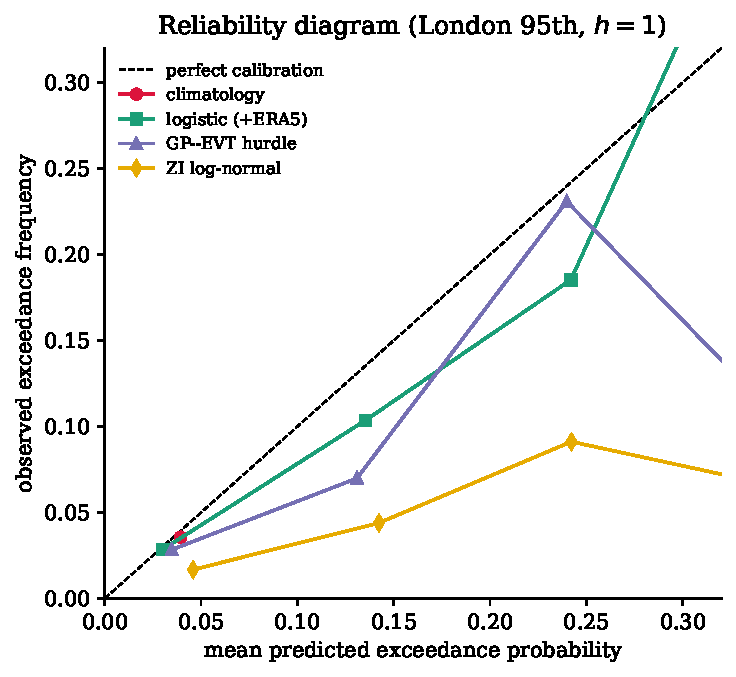
\includegraphics[width=0.62\linewidth]{figures/fig_reliability}
\caption{Reliability diagram for the exceedance probability (London $95$th,
$h{=}1$). The logistic regression and the GP--EVT hurdle track the
diagonal (calibrated) and spread their predictions (informative); the
zero-inflated log-normal is systematically overconfident (its predicted
exceedance probabilities exceed the observed frequencies), despite attaining
nominal conformal coverage by construction. Climatology is a single point
at the base rate. The Paris counterpart is Supplementary Figure~S2.}
\label{fig:reliability}
\end{figure}

\subsection{Predictability of occurrence}\label{sec:res-occ}
Occurrence is weakly but genuinely predictable in both cities: the best calibrated
model improves on climatology with a Brier skill of $+0.038$ in London and
$+0.117$ in the more convective Paris (Table~\ref{tab:bakeoff}), with positive
resolution. An $L_1$-regularised logistic identifies physically sensible
antecedent predictors --- led by the \textbf{K-index} of convective instability,
the $500$\,hPa geopotential, integrated vapour transport, low-level humidity, and
season --- and stability selection confirms their robustness: the K-index and the
most recent index lag are selected in essentially every training subsample (full
ranking, both cities: Supplementary Table~S2). Skill nonetheless decays toward
the prevalence floor as the forecast horizon grows (Figure~\ref{fig:horizon}a;
numerical BSS by horizon, both cities: Supplementary Table~S3), consistent with
the limited day-scale persistence of
these extremes. At the rarer $99$th-percentile threshold (London), where the
scarce data preclude the held-out intensity test, the qualitative picture is
unchanged (Supplementary Table~S1).

\subsection{Predictability of intensity}\label{sec:res-int}
Whether the \emph{magnitude} of an extreme is predictable is the more delicate
question, and the answer is a qualified yes --- in both cities. On the extreme
days, many antecedent features correlate with the excess far beyond chance, and
the association survives multiplicity control: $21$ of $49$ features in London and
$27$ of $49$ in Paris pass a Benjamini--Hochberg false-discovery threshold (versus
$\sim2$ expected), led by convective inhibition and CAPE in both. To test whether
this signal generalises out of sample, we fit quantile regressions of the excess
on held-out extreme days (regularisation chosen by cross-validation on the
training set only) and score them by the CRPS of the excess against the
climatological excess distribution. Computed over a fine quantile grid on the
primary split, the CRPS skill is small but its moving-block bootstrap interval
\emph{excludes zero} in each city (London $+0.014$, $[+0.009,+0.019]$; Paris
$+0.036$, $[+0.005,+0.074]$). As a robustness check we recompute it over a coarser
quantile grid across four independent expanding-window splits per city: the skill
stays positive throughout --- every interval excluding zero, with primary-split
(2009--2018) values of $+0.035$ in each city (Table~\ref{tab:intensity},
Figure~\ref{fig:intensity}). The signal is concentrated in the upper tail (the
largest events) and is carried by antecedent convective instability (CAPE/CIN);
median magnitude is indistinguishable from climatology. The Paris point estimates
run somewhat higher than London's, but their confidence intervals overlap, so we
read the intensity signal as robustly \emph{replicated} across the two cities
rather than decisively stronger in either.

\begin{figure}[t]
\centering
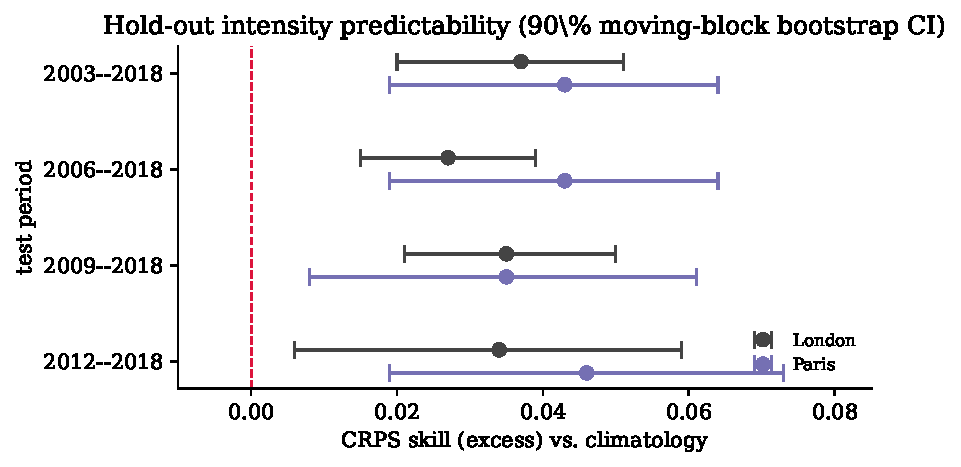
\includegraphics[width=0.72\linewidth]{figures/fig_intensity}
\caption{Hold-out intensity predictability for both cities: CRPS-of-excess skill
over climatology, with $90\%$ moving-block bootstrap intervals, across four
forward-only expanding-window train/test splits. The skill is small but its
interval excludes zero in every split and city; Paris point estimates run somewhat
higher than London's, though the intervals overlap.}
\label{fig:intensity}
\end{figure}

\begin{table}[t]
\centering\small
\caption{Hold-out intensity predictability in both cities: CRPS-of-excess skill
over climatology across forward-only expanding-window splits, with $90\%$
moving-block bootstrap intervals. Every interval excludes zero; Paris point
estimates run somewhat higher than London's, though the intervals overlap.}
\label{tab:intensity}
\begin{tabular}{lcccc}
\toprule
\textbf{Test period} & \textbf{\# test ext.} & \textbf{CRPS skill} & \textbf{$90\%$ CI} & \textbf{P($>0$)} \\
\midrule
\multicolumn{5}{l}{\emph{London}}\\
2003--2018 & $213$ & $+0.037$ & $[+0.020,+0.051]$ & $1.00$ \\
2006--2018 & $175$ & $+0.027$ & $[+0.015,+0.039]$ & $1.00$ \\
2009--2018 & $130$ & $+0.035$ & $[+0.021,+0.050]$ & $1.00$ \\
2012--2018 & $\phantom{0}96$ & $+0.034$ & $[+0.006,+0.059]$ & $0.97$ \\
\midrule
\multicolumn{5}{l}{\emph{Paris}}\\
2003--2018 & $329$ & $+0.043$ & $[+0.019,+0.064]$ & $1.00$ \\
2006--2018 & $275$ & $+0.043$ & $[+0.019,+0.064]$ & $1.00$ \\
2009--2018 & $211$ & $+0.035$ & $[+0.008,+0.061]$ & $0.99$ \\
2012--2018 & $164$ & $+0.046$ & $[+0.019,+0.073]$ & $0.99$ \\
\bottomrule
\end{tabular}
\end{table}

\subsection{Coupling the hurdle: a null result}\label{sec:res-synth}
We also tested whether \emph{coupling} the occurrence and intensity halves of the
hurdle through coregionalisation (Section~\ref{sec:models}) improves forecasts,
and found it weakly identified and empirically inert at this data volume ---
switching the coupling off leaves the bake-off skill unchanged --- so we retain it
only as a harmless nested generalisation of the independent hurdle; the full
synthetic-recovery, misspecification, and real-data $\widehat\rho$ analyses are in
Supplementary Section~S4.

\subsection{Skill decays with horizon}\label{sec:res-skill}
Both occurrence skill and discrimination decay toward the climatological floor as
the forecast horizon grows (Figure~\ref{fig:horizon}a), consistent with the
limited day-scale persistence of London extremes; conformal coverage, being
guaranteed by construction, is flat across horizons (Figure~\ref{fig:horizon}b).
The $+$ERA5 drivers lift discrimination clearly at $h=1$ (PR-AUC $0.118$ versus
$0.076$ for index history alone) but the edge fades into seed noise by $h=3$ --- a
reminder that the predictability documented above is a short-lead effect, weak and
easily masked unless assessed with seed-averaging and proper scores rather than
single runs. The same decay and flat coverage hold for Paris (Supplementary
Figure~S3).

\begin{figure}[t]
\centering
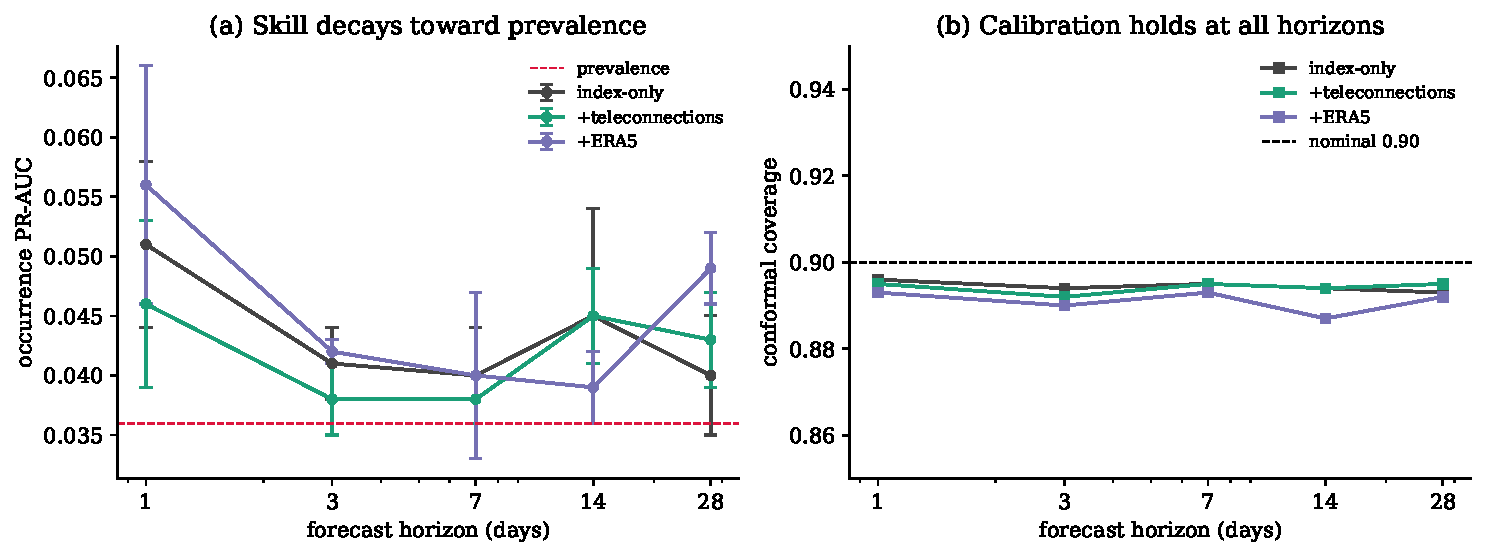
\includegraphics[width=\linewidth]{figures/fig_horizon}
\caption{Seed-averaged horizon sweep on the London $95$th-percentile index
(GP--EVT hurdle). \textbf{(a)} Occurrence PR-AUC decays toward the prevalence floor
(dashed) as the forecast horizon grows; the $+$ERA5 driver gain is clearest at
$h=1$ and fades into seed noise by $h=3$.
\textbf{(b)} Conformal coverage stays at the nominal $0.90$ across all horizons
and predictor sets. Error bars / markers are means over three seeds. The Paris
counterpart is Supplementary Figure~S3.}
\label{fig:horizon}
\end{figure}

\paragraph{Synthesis.} Across the bake-off, a GP--EVT hurdle is the strongest
full-distribution forecaster while simple calibrated models match it on
occurrence, and the response distribution matters as much as the model class
(Section~\ref{sec:res-bakeoff}); conformal coverage holds but is, on
its own, uninformative about forecast quality (Section~\ref{sec:res-cal}). The
substantive finding is a small but
\emph{rigorously established} predictability: occurrence is weakly predictable
from antecedent convective-instability and circulation indices
(Section~\ref{sec:res-occ}), and the magnitude of the largest events is weakly
predictable from antecedent convective instability, with a CRPS skill over
climatology that excludes zero across four independent splits
(Section~\ref{sec:res-int}). The optional dependent-hurdle coupling, tested
separately, proves empirically inert at this data volume
(Section~\ref{sec:res-synth}). Every one of these
conclusions holds in \emph{both} London and Paris, and is generally more
pronounced in the more convective Paris --- evidence that they reflect the
meteorology of precipitation extremes rather than the idiosyncrasies of one city.

% ===========================================================================
\section{Discussion}\label{sec:discussion}
% ===========================================================================

\paragraph{Predictability is real but small, and physically interpretable.}
The headline is not a forecasting triumph but an honest measurement: in both
cities, the occurrence of a daily precipitation extreme and the magnitude of the
largest events carry weak antecedent predictability, on the order of a few percent
of CRPS skill over climatology. Such effect sizes are modest but not unusual for
precipitation at these lead times --- sub-seasonal precipitation forecast skill is
itself typically small --- and their practical value lies less in a sharp point
forecast than in \emph{trustworthy, calibrated} probabilities, plus a slim but
real edge for anticipating the most intense events. That the signal is led by
convective-instability indices (the K-index for occurrence; CAPE and convective
inhibition for intensity) is reassuring: it is the thermodynamics one would expect
to govern intense convective rainfall, it argues against the skill being an
artefact, and it is precisely why the effects are \emph{larger in the more
convective Paris}. The median magnitude of an extreme, by contrast, is
indistinguishable from climatology: once an exceedance occurs, its size is largely
unpredictable except in the upper tail. One nuance reinforces the data-dependence
of these statements: in data-scarcer London no model beats the empirical
climatological tail on the full-predictive score, but in Paris --- with half again
as many extremes --- the extended GPD does, so ``the tail is climatology-bound''
is a sample-size effect, not a universal law.

\paragraph{Methodological lessons.} Three are worth emphasising. First,
\emph{a compact, well-matched model was enough}: in both cities a single-layer
Gaussian-process hurdle with a standard kernel and an EVT tail was the strongest
full-distribution forecaster on the tail, yet on occurrence it was matched by an
inexpensive logistic regression and gradient-boosted trees --- so raw model
sophistication bought little, and a modest Gaussian process is about as much
flexibility as this low-signal problem can bear. Where Gaussian processes would
earn more of their keep is through structure the single-site temporal problem does
not provide (notably spatial structure across the grid of cells). Second, the
\emph{response distribution dominates}: a log-normal tail was substantially
miscalibrated, and hurdling at the extreme threshold starved the tail of data;
modelling the full zero-inflated distribution with a threshold-free extended GPD
was far better. Third, and most relevant to the wider literature, \emph{conformal
coverage is insufficient as a stand-alone indicator of forecast quality}: it is
attained by construction even by a model worse than climatology on proper scores
(the zero-inflated log-normal here). This is a known property of coverage, but our
experiments make it concrete --- reporting coverage without a proper-score
comparison can create a false impression of a good probabilistic forecast.

\paragraph{One predictive distribution, not two analyses.} We report occurrence
and intensity separately for interpretability, but they are not disconnected: they
are the point-mass and tail components of a single hurdle predictive distribution,
$F(z)=(1-\pi)+\pi\,H(z-u)$, with occurrence probability $\pi(\mathbf{x})$ and a
covariate-dependent excess law $H$. Because the (unstructured) hurdle likelihood
factorises in these parameters, fitting the two components jointly is \emph{equivalent}
to fitting them separately --- they are orthogonal pieces of one distribution rather
than two ad hoc models --- and a single threshold-weighted CRPS over $F$ decomposes
additively into an occurrence and an intensity contribution. Fitting this unified
hurdle directly and scoring it end-to-end (Appendix~\ref{app:unified}) recovers
exactly the two-part story: in both cities the overall skill splits into a modest
occurrence term and a small but unusually stable intensity term (its bootstrap
interval excludes zero in both cities), with negligible interaction. The only way
to make the joint fit differ from the separate one is to \emph{couple} the
components through shared latent structure --- the dependent GP hurdle. We tested
this coupling and found it empirically inert at this data volume (Supplementary
Section~S4): the coupled and independent hurdles score identically, and $\rho$ is
too weakly identified on real data to estimate reliably. The separable
(independent) treatment is therefore the well-identified reference, and the
coupling is retained only as a harmless nested generalisation that reduces to it
as $\rho\to0$; whether a richer dataset could make borrowing strength pay is left
open.

\paragraph{Why rigour mattered here.} Several apparent results did not survive
scrutiny: a single-seed driver benefit and an apparent long-horizon gain both
evaporated under seed-averaging, and an across-the-board intensity skill shrank to
an upper-tail effect once regularisation was chosen without peeking at the test
set. The predictability we report is what remained after seed-averaging, proper
scoring, cross-validated model selection, bootstrap intervals, and multi-split
robustness. In a low-signal regime these safeguards are not optional --- they are
the difference between a finding and an artefact.

\paragraph{Limitations.} Four limitations qualify these conclusions.
\begin{itemize}[leftmargin=1.3em,itemsep=4pt]
\item \textbf{Sample size and independence.} The study covers two cities ---
a step beyond a single site, but still a limited sample of European urban
climates, so we frame the results as a careful two-city assessment rather than
a continent-wide claim. London and Paris also share a climate zone, a
downscaled reanalysis product (ERA5-2km), and a data provider (Copernicus), so
they are not fully independent replicates: common reanalysis biases could in
principle inflate both cities' apparent skill together. Replication in a
climatically distinct setting (Mediterranean or continental-interior) would be
needed to rule this out, and we flag it as the most direct next step rather
than a claim we can settle here.
\item \textbf{Perfect-prognosis framing.} The study uses a perfect-prognosis
design (antecedent reanalysis fields, not operational forecasts), and the
intensity analysis conditions on observed exceedances, so it isolates
predictability rather than delivering an end-to-end warning.
\item \textbf{Threshold definitions and stationarity.} The extreme-day
definition itself has two distinct knobs --- the standardisation percentile
$q$ (Section~\ref{sec:data-index}) and the exceedance threshold $u$ applied to
the standardised index (Section~\ref{sec:setup}) --- and we vary each
separately (the $99$th-percentile analysis in the Supplementary Material, and
the $u$-sensitivity check of Section~\ref{sec:res-bakeoff}) rather than
conflating them. We also treat the 1989--2018 climatological reference as
stationary; given that climate projections indicate a rising trend in extreme
rainfall over this period \citep{ipcc2021}, a non-stationary reference (e.g.\
a smoothly time-varying baseline rate) could in principle sharpen or shift the
skill scores reported here. We did not pursue this because the sample is
already short relative to the rarity of the events, making an additional
non-stationary component hard to fit reliably; we flag it as a natural
extension rather than a design choice we defend as final.
\item \textbf{Circularity of the response.} The index is itself an
ERA5-derived precipitation product, which raises a circularity concern. We
address it in two ways: no precipitation field of any kind enters the
predictors, and every driver is strictly lagged, so the predictors are
antecedent dynamical and thermodynamic state (pressure, geopotential,
humidity, instability), never the rainfall itself. Using antecedent state to
predict future precipitation is the standard perfect-prognosis setting; the
residual caveat --- that a reanalysis is internally consistent across
variables and time --- cannot make a strictly-lagged, non-precipitation
predictor circular, but is worth keeping in mind, and would be removed
entirely by moving to numerical-weather-prediction forecast drivers (future
work).
\end{itemize}

% ===========================================================================
\section{Conclusion}\label{sec:conclusion}
% ===========================================================================

We set out to measure, rather than merely to model, the predictability of rare
precipitation extremes, and to do so with an evaluation protocol robust to the
pitfalls of a low-signal setting. The answer, consistent across two climatically
contrasting cities, is a qualified, quantified ``a little'': occurrence and the
magnitude of the largest events are weakly but genuinely predictable from
antecedent convective instability, while a compact Gaussian-process extreme-value
hurdle proves the strongest full-distribution forecaster --- though simple
calibrated models match it on occurrence --- and conformal coverage is no
substitute for a proper-score comparison. That every
finding holds in --- and is generally more pronounced in --- the more convective
Paris is itself evidence that these are properties of precipitation extremes, not
of one city.
Natural extensions are the directions in which more signal, and a genuine role for
structured Gaussian-process models, are most plausible: more cities to map the
predictability across climates, \emph{spatial} modelling across the grid of cells,
\emph{operational} drivers from numerical weather prediction in place of
reanalysis, and \emph{sub-seasonal} aggregations where slowly varying drivers may
contribute. Whether predictability rises materially in those settings is, in the
spirit of this paper, a question to be settled by proper scores and confidence
intervals rather than asserted.

% ===========================================================================
\section*{Data and code availability}\label{sec:availability}
\addcontentsline{toc}{section}{Data and code availability}
% ===========================================================================
The underlying data are publicly available: the London and Paris
precipitation-extreme indices derive from the Copernicus Climate Data Store
product \emph{Extreme precipitation risk indicators for Europe and European cities
(1950--2019)}, and the atmospheric predictors from ERA5 (Copernicus CDS,
\texttt{reanalysis-era5-single-levels}; and the WeatherBench2 regridded ERA5
archive) and from the NOAA teleconnection indices. The code accompanying this
paper --- implementations of all models (logistic, gradient-boosted trees, the
zero-inflated log-normal/gamma/eGPD distributional regressions, and the
GP--EVT hurdle), the full evaluation protocol (proper scores, the hold-out
intensity test, moving-block bootstrap and multi-split robustness), the
data-retrieval and feature-processing scripts, and the scripts that produce every
figure and table --- together with the processed daily feature tables for both
cities, are publicly available at
\url{https://github.com/olatunjijohnson/precip-extremes-predictability}.
Following journal policy, the processed data files will additionally be deposited
on figshare with a citable DOI upon acceptance.

% ===========================================================================
\section*{Author contributions}
% ===========================================================================
\textbf{Olatunji Johnson} is the sole author and is responsible for all
aspects of this work: conceptualisation, methodology, software, formal
analysis, and writing.

% ===========================================================================
\section*{Funding}
% ===========================================================================
This research received no
specific grant from any funding agency in the public, commercial, or
not-for-profit sectors.

% ===========================================================================
\section*{Conflict of interest}
% ===========================================================================
The authors declare no conflict of interest.

% ===========================================================================
\appendix
\section*{Appendix}
% ===========================================================================
\section{Data and predictors}\label{app:data}

\paragraph{Response.} The standardised daily precipitation-extreme index for
London and Paris (Section~\ref{sec:data}), derived from the ERA5-2km downscaled
reanalysis; we use the daily maximum over each city's grid cells ($53$ for London,
$157$ for Paris), with an extreme defined by $\Ind>1$. We analyse the
$95$th-percentile standardisation for both cities and, for London only, the rarer
$99$th percentile (Supplementary Material).

\paragraph{Antecedent predictors.} All predictors are functions of information up
to the forecast origin $t$ (a horizon-$h$ forecast of day $t+h$ uses day-$t$
information only); no precipitation field is used, since the response is itself an
ERA5-derived precipitation product.
\begin{itemize}[leftmargin=1.3em,itemsep=1pt]
\item \textbf{Index history:} lags $\Ind_{t-1},\dots,\Ind_{t-14}$; rolling mean
over the previous $7$ and $30$ days; rolling maximum over $7$ days; count of
exceedances in the previous $30$ days; and $\sin/\cos$ harmonics of day-of-year.
\item \textbf{ERA5 circulation and moisture} (WeatherBench2, $1.5^\circ$, daily
means over a city-centred synoptic box, $\sim15^\circ\times30^\circ$ --- e.g.\
$45$--$60^\circ$N, $20^\circ$W--$10^\circ$E for London, shifted south-east for
Paris): mean sea-level pressure and its meridional/zonal gradients, total-column water
vapour, $2$\,m temperature, $10$\,m wind components and speed, geopotential at
$500$ and $850$\,hPa, and specific humidity at $850$\,hPa.
\item \textbf{ERA5 convective instability} (Copernicus CDS,
\texttt{reanalysis-era5-single-levels}, $0.25^\circ$, daily mean and maximum over
the box): convective available potential energy (CAPE), convective inhibition
(CIN), the K-index, the Total-Totals index,
total-column water vapour, the vertical-integral eastward/northward
water-vapour-flux components and their magnitude (IVT).
\item \textbf{Teleconnection indices} (monthly, broadcast to daily): North
Atlantic Oscillation and Arctic Oscillation (NOAA CPC), and Ni\~no\,3.4 (NOAA PSL).
\end{itemize}

\paragraph{Retrieval.} WeatherBench2 fields were read directly from the public
Google Cloud zarr store with \texttt{xarray}; the convective-instability fields
were retrieved from the Copernicus CDS via \texttt{cdsapi} with server-side
spatial subsetting to the box, $6$-hourly sampling aggregated to daily statistics;
teleconnection indices were downloaded from NOAA. Every driver is forward-filled
to daily resolution where needed and lagged by the forecast horizon. Processing
code and the cached daily feature table accompany the paper.

\section{The Gaussian-process extreme-value hurdle: inference}\label{app:inference}

We give the inference for the Gaussian-process--EVT hurdle
(Section~\ref{sec:models}).
The parameters depend on covariates through latent functions,
$\pi=\sigmoid(g_\pi(\bx_t))$, $\sigma=\softplus(g_\sigma(\bx_t))$, and a constant
shape $\xi_0$ (covariate-dependent $\xi$ is an optional extension). For horizon
$h$ the per-day likelihood factorises into occurrence and (on extreme days)
intensity terms,
\begin{equation}\label{eq:like}
p\big(O_t,\Ind_t\mid \bg(\bx_{t-h})\big)
= \pi^{O_t}(1-\pi)^{1-O_t}\,\big[h_{\GPD}(\Ind_t-u;\sigma,\xi_0)\big]^{O_t}
\,\big[f^{\mathrm{blw}}(\Ind_t)\big]^{1-O_t},
\end{equation}
with $h_{\GPD}$ the GPD density and $f^{\mathrm{blw}}$ a zero-inflated positive
density for the sub-threshold regime.

\paragraph{Sparse variational inference.} We place GP priors on
$\bg=(g_\pi,g_\sigma)$ and introduce $M\ll N$ inducing variables $\bu=\bg(\bZ)$
with whitened variational posterior $q(\bu)=\Normal(\bm m,\bm S)$. The evidence
lower bound is
\begin{equation}\label{eq:elbo}
\mathcal{L} = \sum_t \E_{q(\bg(\bx_{t-h}))}\!\big[\log p(O_t,\Ind_t\mid\bg(\bx_{t-h}))\big]
- \KL\!\big(q(\bu)\,\|\,p(\bu)\big),
\end{equation}
the expectation computed by Monte Carlo over the marginal $q(\bg(\bx_{t-h}))$.
Inducing-point inference reduces cost to $\mathcal{O}(NM^2)$; the kernel is a
standard automatic-relevance-determination squared-exponential kernel acting
directly on the covariates, fitted by (doubly-stochastic) variational inference
\citep{salimbeni2017doubly}.
Hyperparameters, inducing inputs/distribution, and $\xi_0$ are
learned jointly by maximising \eqref{eq:elbo}.

\paragraph{Coregionalised (dependent) hurdle.} We couple the two latents through a
linear model of coregionalisation: with $Q$ shared base GPs $f_q\sim\GP(0,k_\theta)$,
$g_a(\bx)=\sum_{q} W_{aq} f_q(\bx)$, so $\operatorname{Cov}(g_a,g_b)=B_{ab}\,k_\theta$
with $\bB=\bm W\bm W^\top$. The correlation
$\rho=B_{\pi\sigma}/\sqrt{B_{\pi\pi}B_{\sigma\sigma}}$ is the borrowing-strength
parameter; a diagonal $\bm W$ recovers the independent hurdle. Because the excess
is observed only on extreme days, $\rho$ is weakly identified, so we use a
weakly-informative prior shrinking $\rho\to0$; we examine its recovery on
synthetic data and its (null) effect on forecasts in Supplementary Section~S4.

\paragraph{Tail-conformal layer.} For an interval at level $1-\alpha$ we use a
conformalised-quantile-regression nonconformity score on the model's predictive
quantiles, $E_t=\max\{\widehat z_{\alpha/2}-\Ind_t,\ \Ind_t-\widehat z_{1-\alpha/2}\}$;
when the required score quantile exceeds what the calibration set resolves we
extrapolate with a GPD fitted to the top $20\%$ of the upper calibration scores
\citep{pasche2025extreme}, and we adapt the level online by \eqref{eq:aci}
(step size $\gamma=0.02$) over an expanding calibration pool that accumulates
test-day scores as the walk-forward evaluation proceeds.

\section{Unified hurdle: one predictive distribution, decomposed}\label{app:unified}

To verify that the separately reported occurrence and intensity analyses are the
two components of one inferential object (Section~\ref{sec:discussion}), we fit a
single hurdle predictive distribution directly,
\[
F(z\mid\bx)=\begin{cases}1-\pi(\bx) & z\le u,\\[2pt]
(1-\pi(\bx))+\pi(\bx)\,H\!\big(z-u;\sigma(\bx),\xi\big) & z>u,\end{cases}
\]
with $\pi(\bx)=\sigmoid(\bm a^\top\bx)$, $\sigma(\bx)=\softplus(\bm b^\top\bx)$,
$H$ the GPD excess law and $\xi$ a covariate-free tail index, fitting all
parameters by a \emph{single} joint hurdle log-likelihood. Because that likelihood
factorises, this is numerically equivalent to the separate fits; the point is the
\emph{evaluation}. We score the whole $F$ with one threshold-weighted CRPS at
$\tau=u$ and attribute its skill over a parametric climatology (constant base rate
$\bar\pi$ plus a stationary GPD tail) by swapping one component at a time:
$S_{\mathrm{occ}}$ uses $\pi(\bx)$ with the climatological tail, $S_{\mathrm{int}}$
uses $\bar\pi$ with $\sigma(\bx)$, and $S_{\mathrm{full}}$ uses both; the
decomposition is additive up to a small interaction. Intervals are moving-block
bootstrap ($90\%$, block $=10$ days, seed-averaged over three fits); the resulting decomposition is reported in
Table~\ref{tab:unified}.

\begin{table}[ht]
\centering
\small
\setlength{\tabcolsep}{4.5pt}
\begin{tabular}{lcc}
\toprule
twCRPS skill vs climatology & London & Paris \\
\midrule
$S_{\mathrm{full}}$ (occurrence $+$ intensity) & $+0.030$ $[+0.002,+0.061]$ & $+0.084$ $[+0.027,+0.135]$ \\
\quad occurrence contribution $S_{\mathrm{occ}}$ & $+0.029$ $[+0.009,+0.050]$ & $+0.075$ $[+0.043,+0.104]$ \\
\quad intensity contribution $S_{\mathrm{int}}$ & $+0.007$ $[+0.005,+0.009]$ & $+0.013$ $[+0.010,+0.017]$ \\
\quad occurrence\,$\times$\,intensity interaction & $-0.005$ & $-0.004$ \\
\midrule
occurrence BSS (unified $\pi$ / standalone logistic) & $+0.036$ / $+0.038$ & $+0.116$ / $+0.117$ \\
\bottomrule
\end{tabular}
\caption{The single hurdle distribution, scored end-to-end, decomposes into the
two findings reported in the main text: a modest occurrence term and a small but
stable intensity term (its bootstrap interval excludes zero in both cities), with
negligible interaction. The unified occurrence probability reproduces the
standalone logistic skill, confirming the components are orthogonal pieces of one
distribution. The intensity contribution is small because it is averaged over all
test days; restricted to the $\sim\!3$--$6\%$ of days that are extreme it matches
the isolated CRPS-of-excess skill of Section~\ref{sec:res-int}.}
\label{tab:unified}
\end{table}

\bibliographystyle{plainnat}
\bibliography{references}

\end{document}
